\documentclass[11pt, letterpaper]{article}
\usepackage{amsmath, amssymb, amsthm}
\usepackage{graphicx}
\usepackage[margin=1in]{geometry}
\usepackage{parskip}
\usepackage{hyperref}
\usepackage{xcolor}

\hypersetup{
    colorlinks=true,
    linkcolor=blue,
    filecolor=magenta,
    urlcolor=cyan,
}

\theoremstyle{definition}
\newtheorem{definition}{Definition}[section]
\newtheorem{theorem}{Theorem}[section]
\newtheorem{proposition}{Proposition}[section]
\newtheorem{lemma}{Lemma}[section]
\newtheorem{corollary}{Corollary}[section]
\newtheorem{remark}{Remark}[section]
\newtheorem{example}{Example}[section]

\newcommand{\R}{\mathbb{R}}
\newcommand{\norm}[1]{\left\lVert#1\right\rVert}
\newcommand{\mat}[1]{\mathbf{#1}} % Matrix notation
\newcommand{\vect}[1]{\mathbf{#1}} % Vector notation
\DeclareMathOperator{\im}{Im}       % Image of a matrix
\DeclareMathOperator{\spn}{span}    % Span of vectors
\DeclareMathOperator{\rank}{rank}   % Rank of a matrix
\DeclareMathOperator{\argmin}{arg\,min} % Arg min
\DeclareMathOperator{\diag}{diag}   % Diagonal matrix

\title{Lecture Notes: Multiple Linear Regression}
\author{Your Friendly Math Teacher}
\date{\today}

\begin{document}

\maketitle

\section{Introduction: Beyond a Single Predictor}

In our previous discussions, we explored how to model a response variable $y$ using a single explanatory variable $x$. While useful, real-world phenomena are often influenced by multiple factors. Multiple linear regression extends the concepts we've learned to handle situations where we have several explanatory variables influencing our response.

\subsection{The Data}

Our dataset now consists of $n$ observations, where each observation $i$ includes $p$ explanatory variables and one response variable:
\[
(x_{i1}, x_{i2}, \dots, x_{ip}, y_i), \quad i = 1, \dots, n
\]. We collect the explanatory variables for the $i$-th observation into a $p$-dimensional vector $\vect{x}_i = (x_{i1}, \dots, x_{ip})^{\top}$. A crucial assumption we'll make throughout is that $n \ge p+1$. We'll see later why this is important for obtaining a unique solution.

\subsection{Visualization Challenges}

Visualizing this data becomes tricky as $p$ increases. For simple linear regression ($p=1$), a 2D scatter plot suffices. For $p=2$, we can manage a 3D plot, showing $x_1$ and $x_2$ on the base plane and $y$ on the vertical axis. Beyond that, direct scatter plots are impractical. However, the underlying mathematical framework elegantly extends.

\section{The Multiple Linear Regression Model}

Our goal is to predict $y$ using a linear combination of *all* the explanatory variables $x_1, \dots, x_p$. The model takes the form:
\[
\hat{y} = \hat{\beta}_0 + \hat{\beta}_1 x_1 + \hat{\beta}_2 x_2 + \dots + \hat{\beta}_p x_p
\]. Here, $\hat{\beta}_0, \hat{\beta}_1, \dots, \hat{\beta}_p$ are the coefficients we need to estimate from the data. $\hat{\beta}_0$ is the intercept, and $\hat{\beta}_j$ ($j=1, \dots, p$) represents the estimated change in $y$ for a one-unit change in $x_j$, holding all other predictors constant.

\subsection{Introducing the Intercept Term}

To simplify notation, we often incorporate the intercept term into the summation. We achieve this by defining a new "zeroth" explanatory variable $x_{i0}$ that is always equal to 1 for every observation $i$. Our feature vector for observation $i$ then becomes $(p+1)$-dimensional: $\vect{x}_i = (x_{i0}, x_{i1}, \dots, x_{ip})^{\top} = (1, x_{i1}, \dots, x_{ip})^{\top}$. With this convention, the predicted value for the $i$-th observation is:
\[
\hat{y}_i = \hat{\beta}_0 x_{i0} + \hat{\beta}_1 x_{i1} + \dots + \hat{\beta}_p x_{ip} = \sum_{j=0}^{p} \hat{\beta}_j x_{ij}
\].

\subsection{Fitted Values and Residuals}

Just like in simple regression, for any estimated set of coefficients $\hat{\vect{\beta}} = (\hat{\beta}_0, \dots, \hat{\beta}_p)^{\top}$, we can calculate:
\begin{itemize}
    \item \textbf{Fitted values} ($\hat{y}_i$): The model's prediction for observation $i$, given by $\hat{y}_i = \sum_{j=0}^{p} \hat{\beta}_j x_{ij}$.
    \item \textbf{Residuals} ($e_i$): The difference between the observed value and the fitted value, $e_i = y_i - \hat{y}_i$. These represent the prediction errors.
\end{itemize}

\section{The Method of Least Squares}

How do we find the "best" coefficients $\hat{\beta}_0, \dots, \hat{\beta}_p$? We generalize the method of least squares: we seek the coefficients that minimize the sum of the squared residuals (SSR).

\begin{definition}[Least Squares Criterion]
Let $\vect{b} = (b_0, b_1, \dots, b_p)^{\top} \in \R^{p+1}$ be a vector of candidate coefficients. The sum of squared residuals function is:
\[
Q(\vect{b}) = \sum_{i=1}^{n} (y_i - \hat{y}_i)^2 = \sum_{i=1}^{n} \left( y_i - \sum_{j=0}^{p} b_j x_{ij} \right)^2
\]. The least squares estimate $\hat{\vect{\beta}}$ is the vector $\vect{b}$ that minimizes $Q(\vect{b})$.
\end{definition}

\subsection{Finding the Minimum: The Normal Equations}

$Q(\vect{b})$ is a differentiable function of the $p+1$ variables $b_0, \dots, b_p$. To find the minimum, we take the partial derivative with respect to each coefficient $b_r$ and set it to zero.
First, note that for a fixed $i$ and $r$:
\[
\frac{\partial}{\partial b_r} \left( \sum_{j=0}^{p} b_j x_{ij} \right) = x_{ir}
\]. Using the chain rule for differentiation:
\[
\frac{\partial Q}{\partial b_r} = \sum_{i=1}^{n} 2 \left( y_i - \sum_{j=0}^{p} b_j x_{ij} \right) \cdot \left( - \frac{\partial}{\partial b_r} \sum_{j=0}^{p} b_j x_{ij} \right) = -2 \sum_{i=1}^{n} \left( y_i - \sum_{j=0}^{p} b_j x_{ij} \right) x_{ir}
\]. Setting $\frac{\partial Q}{\partial b_r} = 0$ for each $r = 0, 1, \dots, p$, we get:
\[
\sum_{i=1}^{n} \left( y_i - \sum_{j=0}^{p} b_j x_{ij} \right) x_{ir} = 0
\]
Rearranging this gives:
\[
\sum_{i=1}^{n} x_{ir} y_i = \sum_{i=1}^{n} x_{ir} \sum_{j=0}^{p} b_j x_{ij} = \sum_{j=0}^{p} \left( \sum_{i=1}^{n} x_{ir} x_{ij} \right) b_j
\]
This yields a system of $p+1$ linear equations for the $p+1$ unknown coefficients $b_0, \dots, b_p$.

\begin{definition}[Normal Equations (Scalar Form)]
The set of equations that determine the least squares coefficients $\vect{b}$ is:
\[
\sum_{j=0}^{p} \left( \sum_{i=1}^{n} x_{ir} x_{ij} \right) b_j = \sum_{i=1}^{n} x_{ir} y_i, \quad \text{for } r = 0, 1, \dots, p
\]. The solution to this system, if unique, gives the least squares estimate $\hat{\vect{\beta}}$.
\end{definition}

\section{Matrix Formulation}

Writing these equations individually is cumbersome. Linear algebra provides a much more compact and insightful representation.

\subsection{Key Matrices and Vectors}

Let's define the following:
\begin{itemize}
    \item \textbf{Response vector} $\vect{y} \in \R^n$: The vector of observed responses.
    \[
    \vect{y} = \begin{pmatrix} y_1 \\ y_2 \\ \vdots \\ y_n \end{pmatrix}
    \]
   .
    \item \textbf{Design Matrix} $\mat{X} \in \R^{n \times (p+1)}$: The matrix whose rows are the feature vectors (including the leading 1 for the intercept) for each observation.
    \[
    \mat{X} = \begin{pmatrix}
    x_{10} & x_{11} & \cdots & x_{1p} \\
    x_{20} & x_{21} & \cdots & x_{2p} \\
    \vdots & \vdots & \ddots & \vdots \\
    x_{n0} & x_{n1} & \cdots & x_{np}
    \end{pmatrix} = \begin{pmatrix}
    1 & x_{11} & \cdots & x_{1p} \\
    1 & x_{21} & \cdots & x_{2p} \\
    \vdots & \vdots & \ddots & \vdots \\
    1 & x_{n1} & \cdots & x_{np}
    \end{pmatrix}
    \]
   . The $i$-th row is $\vect{x}_i^{\top}$. The $j$-th column, denoted $\vect{X}_j$, contains all $n$ observations for the $j$-th predictor $(j=1, \dots, p)$. The 0-th column $\vect{X}_0$ is a vector of all ones, $\vect{1}_n$.
    \item \textbf{Coefficient vector} $\vect{b} \in \R^{p+1}$: The vector of coefficients we want to estimate.
    \[
    \vect{b} = \begin{pmatrix} b_0 \\ b_1 \\ \vdots \\ b_p \end{pmatrix}
    \]
   .
\end{itemize}

\subsection{Normal Equations in Matrix Form}

Now, let's look at the terms in the scalar normal equations:
\begin{itemize}
    \item $\sum_{i=1}^{n} x_{ir} x_{ij}$: This is the dot product of the $r$-th column of $\mat{X}$ and the $j$-th column of $\mat{X}$. This is precisely the element at row $r$, column $j$ of the matrix product $\mat{X}^{\top}\mat{X}$. That is, $(\mat{X}^{\top}\mat{X})_{rj} = \sum_{i=1}^{n} x_{ir} x_{ij}$.
    \item $\sum_{i=1}^{n} x_{ir} y_i$: This is the dot product of the $r$-th column of $\mat{X}$ and the vector $\vect{y}$. This is the $r$-th element of the vector $\mat{X}^{\top}\vect{y}$. That is, $(\mat{X}^{\top}\vect{y})_r = \sum_{i=1}^{n} x_{ir} y_i$.
\end{itemize}
Substituting these into the scalar normal equations $\sum_{j=0}^{p} (\mat{X}^{\top}\mat{X})_{rj} b_j = (\mat{X}^{\top}\vect{y})_r$ for $r=0, \dots, p$, we recognize this as the definition of matrix-vector multiplication.

\begin{theorem}[Normal Equations (Matrix Form)]
The system of normal equations in matrix form is:
\[
(\mat{X}^{\top}\mat{X}) \vect{b} = \mat{X}^{\top}\vect{y}
\].
\end{theorem}

This is a compact equation for the vector $\vect{b}$!

\subsection{Solving for the Coefficients}

The equation $(\mat{X}^{\top}\mat{X}) \vect{b} = \mat{X}^{\top}\vect{y}$ is a standard linear system $A\vect{x} = \vect{c}$, where $A = \mat{X}^{\top}\mat{X}$ is a $(p+1) \times (p+1)$ square matrix, $\vect{x} = \vect{b}$, and $\vect{c} = \mat{X}^{\top}\vect{y}$.

A unique solution exists if and only if the matrix $\mat{X}^{\top}\mat{X}$ is invertible. When is this true?
\begin{itemize}
    \item $\mat{X}^{\top}\mat{X}$ is invertible if and only if the columns of the design matrix $\mat{X}$ are linearly independent. This means no predictor column (including the column of ones) can be written as a linear combination of the others.
    \item A necessary condition for the columns of $\mat{X} \in \R^{n \times (p+1)}$ to be linearly independent is that the number of columns does not exceed the number of rows, i.e., $p+1 \le n$. This is the assumption we made earlier! If $p+1 > n$, the columns *must* be linearly dependent, $\mat{X}^{\top}\mat{X}$ is singular (not invertible), and the system has infinitely many solutions. The least squares coefficients are not unique in this case.
    \item Assuming $p+1 \le n$, linear independence usually holds unless there's perfect multicollinearity (one predictor is an exact linear function of others) or a predictor is constant (and thus a multiple of the intercept column).
\end{itemize}

\begin{theorem}[Least Squares Solution]
If the columns of the design matrix $\mat{X}$ are linearly independent (which implies $p+1 \le n$ and requires $\mat{X}^{\top}\mat{X}$ to be invertible), the unique least squares estimate $\hat{\vect{\beta}}$ is given by:
\[
\hat{\vect{\beta}} = (\mat{X}^{\top}\mat{X})^{-1} \mat{X}^{\top}\vect{y}
\].
\end{theorem}

\begin{remark}
From now on, we will generally assume the columns of $\mat{X}$ are linearly independent, ensuring a unique solution exists.
\end{remark}

\section{Geometric Interpretation}

There's a beautiful geometric way to understand the least squares solution, connecting it to concepts from linear algebra like vector spaces and projections.

\subsection{Linear Algebra Preliminaries}

Let's refresh some key ideas:
\begin{itemize}
    \item \textbf{Image (Column Space)}: For an $n \times m$ matrix $\mat{A}$, its image, $\im(\mat{A})$, is the subspace of $\R^n$ spanned by its columns $\vect{A}_1, \dots, \vect{A}_m$. It's the set of all possible vectors you can form by linear combinations $A\vect{v}$ for $\vect{v} \in \R^m$. We often call this the column space, denoted $colsp(\mat{A})$.
    \item \textbf{Inner Product}: For $\vect{u}, \vect{v} \in \R^n$, the standard inner product (dot product) is $\vect{u}^{\top}\vect{v} = \sum_{i=1}^n u_i v_i$.
    \item \textbf{Norm}: The Euclidean norm (length) of $\vect{v}$ is $\norm{\vect{v}} = \sqrt{\vect{v}^{\top}\vect{v}} = \sqrt{\sum v_i^2}$. The distance between $\vect{u}$ and $\vect{v}$ is $\norm{\vect{u}-\vect{v}}$.
    \item \textbf{Orthogonality}: $\vect{u}$ is orthogonal to $\vect{v}$ ($\vect{u} \perp \vect{v}$) if $\vect{u}^{\top}\vect{v} = 0$.
    \item \textbf{Orthogonal Complement}: For a subspace $M \subseteq \R^n$, its orthogonal complement $M^{\perp}$ is the subspace of all vectors orthogonal to *every* vector in $M$: $M^{\perp} = \{ \vect{v} \in \R^n \mid \vect{v}^{\top}\vect{u} = 0 \text{ for all } \vect{u} \in M \}$.
    \item \textbf{Pythagorean Theorem}: If $\vect{u} \perp \vect{v}$, then $\norm{\vect{u}+\vect{v}}^2 = \norm{\vect{u}}^2 + \norm{\vect{v}}^2$.
\end{itemize}

\subsection{Least Squares as Projection}

Recall the least squares objective function $Q(\vect{b}) = \sum_{i=1}^{n} (y_i - \sum_{j=0}^{p} b_j x_{ij})^2$. Let $\hat{\vect{y}} = \mat{X}\vect{b}$ be the vector of predicted values corresponding to the coefficient vector $\vect{b}$. Then we can write the objective function using vector norms:
\[
Q(\vect{b}) = \sum_{i=1}^{n} (y_i - \hat{y}_i)^2 = \norm{\vect{y} - \hat{\vect{y}}}^2 = \norm{\vect{y} - \mat{X}\vect{b}}^2
\].
Minimizing $Q(\vect{b})$ means finding the vector $\vect{b}$ such that the vector $\hat{\vect{y}} = \mat{X}\vect{b}$ is *closest* to the observed vector $\vect{y}$ in terms of Euclidean distance.

Where do the possible predicted vectors $\hat{\vect{y}} = \mat{X}\vect{b}$ live? Since $\hat{\vect{y}}$ is a linear combination of the columns of $\mat{X}$ (with coefficients given by $\vect{b}$), all possible predicted vectors $\hat{\vect{y}}$ form the column space of $\mat{X}$, $colsp(\mat{X}) = \im(\mat{X})$.

So, the least squares problem is equivalent to finding the vector $\hat{\vect{y}}$ within the subspace $colsp(\mat{X})$ that is closest to the vector $\vect{y}$. Geometrically, this closest vector is the **orthogonal projection** of $\vect{y}$ onto the subspace $colsp(\mat{X})$. Let $\hat{\vect{\beta}}$ be the coefficient vector that produces this projection, so $\hat{\vect{y}} = \mat{X}\hat{\vect{\beta}}$.

\begin{center}
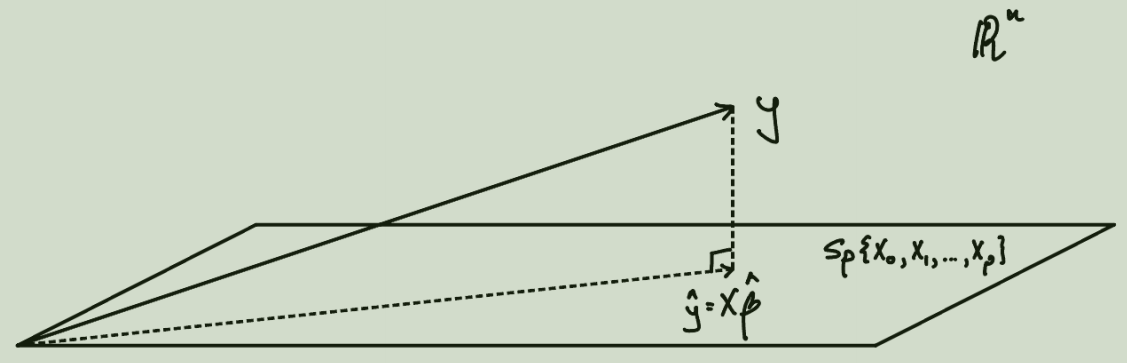
\includegraphics[width=0.6\textwidth]{image1.png}
Figure 1: Geometric interpretation: $\hat{\vect{y}} = \mat{X}\hat{\vect{\beta}}$ is the orthogonal projection of $\vect{y}$ onto the column space of $\mat{X}$ (denoted $Sp\{x_0, ..., x_p\}$ in the diagram).
\end{center}

What defines the orthogonal projection? The vector connecting $\hat{\vect{y}}$ to $\vect{y}$, which is the residual vector $\vect{e} = \vect{y} - \hat{\vect{y}}$, must be orthogonal to the subspace $colsp(\mat{X})$. This means $\vect{e}$ must be orthogonal to every vector in $colsp(\mat{X})$, and in particular, it must be orthogonal to each basis vector of the subspace, i.e., the columns of $\mat{X}$.

Mathematically, the orthogonality condition is $\vect{X}_j^{\top} \vect{e} = 0$ for all $j=0, \dots, p$. We can write this compactly in matrix form:
\[
\mat{X}^{\top} \vect{e} = \vect{0}
\]
Substituting $\vect{e} = \vect{y} - \hat{\vect{y}} = \vect{y} - \mat{X}\hat{\vect{\beta}}$, we get:
\[
\mat{X}^{\top} (\vect{y} - \mat{X}\hat{\vect{\beta}}) = \vect{0}
\]. Rearranging this gives:
\[
\mat{X}^{\top}\vect{y} - \mat{X}^{\top}\mat{X}\hat{\vect{\beta}} = \vect{0} \implies \mat{X}^{\top}\mat{X}\hat{\vect{\beta}} = \mat{X}^{\top}\vect{y}
\]. Look familiar? These are exactly the Normal Equations we derived earlier using calculus!

Assuming again that $\mat{X}^{\top}\mat{X}$ is invertible, we solve for $\hat{\vect{\beta}}$:
\[
\hat{\vect{\beta}} = (\mat{X}^{\top}\mat{X})^{-1} \mat{X}^{\top}\vect{y}
\]. This provides a satisfying geometric intuition for the algebraic solution.

\section{The Projection Matrix (Hat Matrix)}

The vector of fitted values $\hat{\vect{y}}$ is obtained by projecting $\vect{y}$ onto $colsp(\mat{X})$. We can express this projection using a matrix operation.
Substituting the formula for $\hat{\vect{\beta}}$ into $\hat{\vect{y}} = \mat{X}\hat{\vect{\beta}}$, we get:
\[
\hat{\vect{y}} = \mat{X} \left( (\mat{X}^{\top}\mat{X})^{-1} \mat{X}^{\top}\vect{y} \right) = \left( \mat{X} (\mat{X}^{\top}\mat{X})^{-1} \mat{X}^{\top} \right) \vect{y}
\].

\begin{definition}[Projection Matrix / Hat Matrix]
The matrix $\mat{P}_{\mat{X}} \in \R^{n \times n}$ defined as
\[
\mat{P}_{\mat{X}} = \mat{X} (\mat{X}^{\top}\mat{X})^{-1} \mat{X}^{\top}
\]
is the orthogonal projection matrix onto the column space of $\mat{X}$, $colsp(\mat{X})$. It projects any vector $\vect{v} \in \R^n$ onto $colsp(\mat{X})$. The fitted values are given by $\hat{\vect{y}} = \mat{P}_{\mat{X}}\vect{y}$. (It's sometimes called the "hat matrix" because it puts the hat on $\vect{y}$).
\end{definition}

\begin{remark}
This definition assumes $\mat{X}^{\top}\mat{X}$ is invertible (i.e., columns of $\mat{X}$ are linearly independent). The concept of projection still exists even if columns are dependent, but the formula needs adjustment, often by first finding a basis for $colsp(\mat{X})$.
\end{remark}

\subsection{Properties of Projection Matrices}

Let $\mat{P}_{\mat{X}}$ be the projection matrix onto $colsp(\mat{X})$, assuming $\mat{X}$ has full column rank ($p+1$). It has several important properties:

\begin{proposition} Let $\mat{X}$ be $n \times (p+1)$ with linearly independent columns. Then $\mat{P}_{\mat{X}} = \mat{X}(\mat{X}^{\top}\mat{X})^{-1}\mat{X}^{\top}$ satisfies:
\begin{enumerate}
    \item \textbf{Symmetry}: $\mat{P}_{\mat{X}}^{\top} = \mat{P}_{\mat{X}}$.
    \item \textbf{Idempotence}: $\mat{P}_{\mat{X}}^2 = \mat{P}_{\mat{X}}$. (Projecting something already in the subspace doesn't change it).
    \item $\mat{P}_{\mat{X}}\mat{X} = \mat{X}$. (Projecting the columns of $\mat{X}$ onto their own span leaves them unchanged).
    \item $\mat{X}^{\top}(\mat{I} - \mat{P}_{\mat{X}}) = \mat{0}$. (The residual space, associated with $\mat{I}-\mat{P}_{\mat{X}}$, is orthogonal to the column space).
    \item For any $\vect{v} \in \R^n$, $\mat{P}_{\mat{X}}\vect{v} \in \im(\mat{X})$.
    \item If $p+1=n$ (so $\mat{X}$ is square and invertible), then $\mat{P}_{\mat{X}} = \mat{I}_n$.
    \item For any $\vect{v} \in \R^n$, $(\mat{I} - \mat{P}_{\mat{X}})\vect{v} \in \im(\mat{X})^{\perp}$. ($\mat{I}-\mat{P}_{\mat{X}}$ projects onto the orthogonal complement).
    \item If $\vect{w} \in \im(\mat{X})$, then $\mat{P}_{\mat{X}}\vect{w} = \vect{w}$.
    \item If $\vect{w} \in \im(\mat{X})^{\perp}$, then $\mat{P}_{\mat{X}}\vect{w} = \vect{0}$.
    \item $\mat{P}_{\mat{X}}$ depends only on the subspace $\im(\mat{X})$, not the specific basis chosen for it. If $\im(\mat{Z}) = \im(\mat{X})$, then $\mat{P}_{\mat{Z}} = \mat{P}_{\mat{X}}$.
    \item If $L, M$ are subspaces with $L \subseteq M$, then $\mat{P}_M \mat{P}_L = \mat{P}_L \mat{P}_M = \mat{P}_L$. (Projecting onto $L$ then $M$ is the same as just projecting onto $L$).
\end{enumerate}
\end{proposition}
\begin{proof} (Selected proofs, see original notes for others)
\begin{enumerate}
    \item $\mat{P}_{\mat{X}}^{\top} = [\mat{X}(\mat{X}^{\top}\mat{X})^{-1}\mat{X}^{\top}]^{\top} = (\mat{X}^{\top})^{\top} ((\mat{X}^{\top}\mat{X})^{-1})^{\top} \mat{X}^{\top} = \mat{X} (\mat{X}^{\top}\mat{X})^{-1} \mat{X}^{\top} = \mat{P}_{\mat{X}}$. (Used $(\mat{A}^{-1})^{\top} = (\mat{A}^{\top})^{-1}$ and $(\mat{A}\mat{B})^{\top} = \mat{B}^{\top}\mat{A}^{\top}$, and $(\mat{X}^{\top}\mat{X})$ is symmetric).
    \item $\mat{P}_{\mat{X}}^2 = [\mat{X}(\mat{X}^{\top}\mat{X})^{-1}\mat{X}^{\top}] [\mat{X}(\mat{X}^{\top}\mat{X})^{-1}\mat{X}^{\top}] = \mat{X}(\mat{X}^{\top}\mat{X})^{-1} (\mat{X}^{\top}\mat{X}) (\mat{X}^{\top}\mat{X})^{-1}\mat{X}^{\top} = \mat{X}(\mat{X}^{\top}\mat{X})^{-1}\mat{I}\mat{X}^{\top} = \mat{P}_{\mat{X}}$.
    \item $\mat{P}_{\mat{X}}\mat{X} = \mat{X}(\mat{X}^{\top}\mat{X})^{-1}\mat{X}^{\top}\mat{X} = \mat{X}(\mat{X}^{\top}\mat{X})^{-1}(\mat{X}^{\top}\mat{X}) = \mat{X}\mat{I} = \mat{X}$.
\end{enumerate}
\end{proof}

\subsection{Orthogonal Decomposition and Projections}

Projection matrices are fundamental to decomposing vectors relative to a subspace and its orthogonal complement.

\begin{proposition}[Orthogonal Decomposition]
Let $M$ be a subspace of $\R^n$. Any vector $\vect{v} \in \R^n$ can be uniquely represented as $\vect{v} = \vect{w} + \vect{z}$, where $\vect{w} \in M$ and $\vect{z} \in M^{\perp}$. In this decomposition, $\vect{w} = \mat{P}_M \vect{v}$ and $\vect{z} = (\mat{I} - \mat{P}_M)\vect{v} = \mat{P}_{M^{\perp}}\vect{v}$. Furthermore, $\vect{w} = \mat{P}_M \vect{v}$ is the unique vector in $M$ that minimizes the squared distance to $\vect{v}$, i.e., $\vect{w} = \argmin_{\vect{u} \in M} \norm{\vect{v}-\vect{u}}^2$.
\end{proposition}
\begin{proof}
Let $\vect{w} = \mat{P}_M \vect{v}$ and $\vect{z} = \vect{v} - \mat{P}_M \vect{v}$. By properties of $\mat{P}_M$, $\vect{w} \in M$ and $\vect{z} \in M^{\perp}$. Clearly $\vect{v} = \vect{w}+\vect{z}$. For uniqueness, suppose $\vect{v} = \vect{w}_1 + \vect{z}_1 = \vect{w}_2 + \vect{z}_2$ with $\vect{w}_1, \vect{w}_2 \in M$ and $\vect{z}_1, \vect{z}_2 \in M^{\perp}$. Then $\vect{w}_1 - \vect{w}_2 = \vect{z}_2 - \vect{z}_1$. The LHS is in $M$ and the RHS is in $M^{\perp}$. Since the only vector in both $M$ and $M^{\perp}$ is $\vect{0}$, we must have $\vect{w}_1 - \vect{w}_2 = \vect{0}$ and $\vect{z}_2 - \vect{z}_1 = \vect{0}$, so $\vect{w}_1=\vect{w}_2$ and $\vect{z}_1=\vect{z}_2$.
For the minimization property: take any $\vect{u} \in M$. Then $\vect{w}-\vect{u} \in M$, and $\vect{z} \in M^{\perp}$, so $(\vect{w}-\vect{u}) \perp \vect{z}$. By Pythagoras:
\[
\norm{\vect{v}-\vect{u}}^2 = \norm{(\vect{w}+\vect{z})-\vect{u}}^2 = \norm{(\vect{w}-\vect{u}) + \vect{z}}^2 = \norm{\vect{w}-\vect{u}}^2 + \norm{\vect{z}}^2
\]. This is minimized when $\norm{\vect{w}-\vect{u}}^2 = 0$, i.e., when $\vect{u}=\vect{w}$. The minimum value is $\norm{\vect{z}}^2 = \norm{(\mat{I}-\mat{P}_M)\vect{v}}^2$.
\end{proof}

\begin{proposition} We have the following identities:
\begin{enumerate}
    \item $\mat{I} - \mat{P}_{\mat{X}}$ is the projection matrix onto $\im(\mat{X})^{\perp}$. We denote it $\mat{P}_{\im(\mat{X})^{\perp}}$.
    \item If $L \subseteq M$ are subspaces, then $\mat{P}_M - \mat{P}_L$ is the projection matrix onto the subspace $M \cap L^{\perp}$ (the part of $M$ that is orthogonal to $L$).
\end{enumerate}
\end{proposition}

\begin{proposition}
Any symmetric ($\mat{Q}^{\top}=\mat{Q}$) and idempotent ($\mat{Q}^2 = \mat{Q}$) matrix $\mat{Q}$ is the projection matrix onto its own image, $M = \im(\mat{Q})$.
\end{proposition}

\subsection{Spectral Properties of Projection Matrices}

Projection matrices have a particularly simple structure when viewed through their eigenvalues and eigenvectors. Recall:
\begin{itemize}
    \item A symmetric matrix $\mat{A} \in \R^{n \times n}$ is diagonalizable by an orthogonal matrix: $\mat{A} = \mat{U}\mat{D}\mat{U}^{\top}$, where $\mat{U}$ is orthogonal ($\mat{U}^{\top}\mat{U}=\mat{I}$, so $\mat{U}^{-1}=\mat{U}^{\top}$) and $\mat{D}$ is diagonal. The diagonal entries of $\mat{D}$ are the eigenvalues of $\mat{A}$, and the columns of $\mat{U}$ are the corresponding orthonormal eigenvectors. All eigenvalues of a real symmetric matrix are real.
    \item A symmetric matrix $\mat{A}$ is positive semidefinite (PSD) if all its eigenvalues are $\ge 0$. This is equivalent to $\vect{x}^{\top}\mat{A}\vect{x} \ge 0$ for all $\vect{x}$. It is positive definite (PD) if eigenvalues are $> 0$ (equiv. $\vect{x}^{\top}\mat{A}\vect{x} > 0$ for $\vect{x} \ne \vect{0}$).
    \item Any PSD matrix $\mat{A}$ has a unique PSD square root $\mat{B} = \mat{A}^{1/2} = \mat{U}\mat{D}^{1/2}\mat{U}^{\top}$ such that $\mat{B}^2 = \mat{A}$. It can also be written as $\mat{A}=\mat{B}\mat{B}^{\top}$ for some $\mat{B}$ (e.g., $\mat{B}=\mat{U}\mat{D}^{1/2}$).
\end{itemize}

Now, consider a projection matrix $\mat{P}_M$ onto a subspace $M \subseteq \R^n$ with $\dim(M)=m$.
\begin{itemize}
    \item Since $\mat{P}_M$ is symmetric, it's orthogonally diagonalizable: $\mat{P}_M = \mat{U}\mat{D}\mat{U}^{\top}$.
    \item Since $\mat{P}_M$ is idempotent ($\mat{P}_M^2 = \mat{P}_M$), its eigenvalues $\lambda$ must satisfy $\lambda^2 = \lambda$. This means the only possible eigenvalues are $0$ or $1$.
    \item The dimension of the image (column space) is the rank of the matrix, which equals the number of non-zero eigenvalues. Since $\dim(\im(\mat{P}_M)) = \dim(M) = m$, there must be exactly $m$ eigenvalues equal to 1 and $n-m$ eigenvalues equal to 0.
    \item Therefore, the diagonal matrix $\mat{D}$ in the spectral decomposition can be arranged as $\mat{D} = \diag(\underbrace{1, \dots, 1}_{m \text{ times}}, \underbrace{0, \dots, 0}_{n-m \text{ times}})$.
    \item The columns of $\mat{U}$ corresponding to the eigenvalue 1 form an orthonormal basis for the subspace $M = \im(\mat{P}_M)$.
    \item The columns of $\mat{U}$ corresponding to the eigenvalue 0 form an orthonormal basis for the orthogonal complement $M^{\perp} = \ker(\mat{P}_M)$.
    \item Since all eigenvalues are $\ge 0$, $\mat{P}_M$ is positive semidefinite. (It's positive definite only if $m=n$, in which case $\mat{P}_M = \mat{I}_n$).
\end{itemize}
This eigenvalue structure cleanly reflects the geometric action of projection.

\end{document}